\section{两个复形的联结}
\sourcepage{444--445}
本节引入两个复形的联结，并考察它的一些性质。

\entry{定义}{8.2.1}设 $K,L$ 是欧氏空间 $E^J$ 中的非空复形，其一般单形分别写作 $s=v_0\cdots v_m$ 和 $t=w_0\cdots w_n$。假定对任意 $s\in K,t\in L$，点
\[v_0,\ldots,v_m,w_0,\ldots,w_n\]
都仿射无关，记它们张成的单形为
\[s*t=v_0\cdots v_mw_0\cdots w_n.\]
如果所有这样的单形及其面构成单纯复形，就称此复形为 $K$ 与 $L$ 的\emph{联结}（join），记为 $K*L$。

若 $K$ 只有一个顶点 $v$，则 $v*L$ 就是已经定义的 $L$ 上的锥。若 $K$ 由两个点组成，则 $K*L$ 称为 $L$ 的\emph{悬挂}，记为 $S(L)$。下一引理给出一般情形下联结存在的条件。

\entry{引理}{8.2.2}设 $K,L$ 是 $E^J$ 中不交的非空复形。
\begin{enumerate}[label=(\alph*)]
\item 若 $K*L$ 存在，则其多面体等于连接 $|K|$ 中点与 $|L|$ 中点的所有线段的并。任意两条不同的这样的线段至多在一个公共端点相交。
\item 反之，若连接两空间中点的任意两条不同线段至多在一个公共端点相交，则 $K*L$ 存在。
\end{enumerate}

\textbf{证明：}第一步：先证明单形情形。设 $\sigma=v_0\cdots v_mw_0\cdots w_n$，$s=v_0\cdots v_m$，$t=w_0\cdots w_n$。则 $\sigma$ 等于连接 $s$ 中点与 $t$ 中点的所有线段的并，不同的这样的线段至多在公共端点相交；此外，$\Int\sigma$ 等于连接 $\Int s$ 中点与 $\Int t$ 中点的所有开线段的并。这是第 1.2 节的一道习题，现在给出证明。

先证关于内部的断言。若 $p=\lambda x+(1-\lambda)y$，其中 $0<\lambda<1$，$x\in\Int s,y\in\Int t$，写
\[x=\sum\alpha_i v_i,\qquad y=\sum\beta_jw_j,\qquad
\alpha_i,\beta_j>0,\quad\sum\alpha_i=\sum\beta_j=1.\]
则 $p=\sum(\lambda\alpha_i)v_i+\sum(1-\lambda)\beta_jw_j$ 的系数都正且总和为 $1$，故 $p\in\Int\sigma$。反之，若
\[p=\sum\gamma_iv_i+\sum\delta_jw_j\in\Int\sigma,\]
其中所有系数均正、总和为 $1$，令 $\lambda=\sum\gamma_i$，$\alpha_i=\gamma_i/\lambda$，$\beta_j=\delta_j/(1-\lambda)$，则
\[p=\lambda\sum\alpha_iv_i+(1-\lambda)\sum\beta_jw_j,\]
所以 $p$ 位于连接两内部点的开线段上。

再证关于整个单形的断言。$\sigma$ 凸，所以包含所有连接 $s,t$ 中点的线段。反之，若 $x\in\sigma$ 且 $x$ 既不在 $s$ 中也不在 $t$ 中，则 $x$ 位于某个面 $\sigma'$ 的内部，且 $\sigma'$ 与 $s,t$ 都有公共顶点。由刚证明的结论，$x$ 位于连接 $\sigma'\cap s$ 中点与 $\sigma'\cap t$ 中点的开线段上。

最后证明交点性质。若同一点 $p$ 有两种表达
\[
p=\lambda\sum\alpha_iv_i+(1-\lambda)\sum\beta_jw_j
=\lambda'\sum\alpha'_iv_i+(1-\lambda')\sum\beta'_jw_j,
\]
其中 $0\le\lambda,\lambda'\le1$，各重心系数非负，各组和为 $1$，则由顶点仿射无关得到
\[\lambda\alpha_i=\lambda'\alpha'_i,\qquad
(1-\lambda)\beta_j=(1-\lambda')\beta'_j.\]
第一组求和得 $\lambda=\lambda'$。若它等于 $0$ 或 $1$，则 $p$ 是两线段的公共端点；否则各重心系数相等，两线段实际相同。

第二步：证明 (a)。考虑不同线段 $xy,x'y'$，其中
\[x\in\Int s,\quad x'\in\Int s',\quad y\in\Int t,\quad y'\in\Int t',
\qquad s,s'\in K,\quad t,t'\in L.\]
由第一步，
\[xy\subset\Int s\cup\Int(s*t)\cup\Int t,\qquad
x'y'\subset\Int s'\cup\Int(s'*t')\cup\Int t'.\]
\sourcepage{446}
因为 $K*L$ 是复形，若 $s\ne s'$ 且 $t\ne t'$，这些开单形两两不交，故两线段不交。若 $s=s'$ 而 $t\ne t'$，交点只能在 $\Int s$ 中，因此至多是两线段的公共端点。$s\ne s',t=t'$ 的情形同理；若 $s=s',t=t'$，则由第一步得到结论。

第三步：证明 (b)。先证明任意 $s=v_0\cdots v_m\in K$、$t=w_0\cdots w_n\in L$ 的全部顶点仿射无关。考虑线性奇异单形
\[\ell=\ell(v_0,\ldots,v_m,w_0,\ldots,w_n):\Delta_{m+n+1}\to E^J.\]
它把连接 $\epsilon_0\cdots\epsilon_m$ 中点与 $\epsilon_{m+1}\cdots\epsilon_{m+n+1}$ 中点的线段，线性映到连接 $s,t$ 中点的线段。由假设及第一步，$\ell$ 是单射。因此这些顶点张成的仿射平面维数必须是 $m+n+1$，否则 $\ell$ 不可能为单射。所以顶点仿射无关。

还需证明所得单形组成复形。如果两个不同的单形内部相交，除去 $K,L$ 本身已为复形的情形，其中一个必为 $s*t$。$\Int(s*t)$ 中每点都位于连接 $|K|$ 与 $|L|$ 中点的开线段上。如果它与 $\Int(s'*t')$ 相交，就有两条不同开线段相交；如果它与 $\Int s'$ 或 $\Int t'$ 相交，则某条这样的线段的内点同时是另一条的端点。这些都违反假设。因此所得单形确实组成复形。\hfill$\square$

若给定复形 $K,L$ 的欧氏空间位置使联结无法定义，可以找出分别与它们同构的复形 $K_0,L_0$，使 $K_0*L_0$ 存在。例如，可把它们取为某个标准单形 $\Delta^J$ 的两个不交子复形。

\entry{引理}{8.2.3}假设 $K*L$ 存在且 $K$ 局部有限。则
\[
\pi:|K|\times|L|\times I\to|K*L|,\qquad
\pi(x,y,t)=(1-t)x+ty
\]
是商映射。它把每个 $x\times|L|\times0$ 压成一点，把每个 $|K|\times y\times1$ 压成一点，除此之外是一一的。

\textbf{证明：}先用第 2.8 节的结果，证明定义域拓扑由各 $\sigma\times\tau\times I$（$\sigma\in K,\tau\in L$）协调。$|L|\times I$ 的拓扑由各 $\tau\times I$ 协调；$|K|$ 是局部紧 Hausdorff 空间，因此乘积拓扑由各 $|K|\times\tau\times I$ 协调。又因 $\tau\times I$ 局部紧 Hausdorff（事实上紧致），后者的拓扑由各 $\sigma\times\tau\times I$ 协调。故一个集合在整个乘积中闭，当且仅当它与每个这样子空间的交在该子空间中闭。

\sourcepage{447}
按定义，$\pi:\sigma\times\tau\times I\to\sigma*\tau$ 连续，因为二者都有欧氏子空间拓扑。$\sigma*\tau$ 到 $|K*L|$ 的包含也连续，因此 $\pi$ 的各个限制连续。由协调拓扑性质，$\pi$ 连续。

若 $\pi^{-1}(A)$ 闭，则它与每个 $\sigma\times\tau\times I$ 的交闭，因而紧致。其像 $A\cap(\sigma*\tau)$ 紧致，因而闭。于是 $A$ 在 $|K*L|$ 中闭，证明 $\pi$ 是商映射。它恰好实施所述粘合，则由引理 8.2.2 得到。\hfill$\square$

\entry{记号}{8.2.4}用 $X\approx Y$ 表示拓扑空间 $X,Y$ 同胚。

\entry{推论}{8.2.5}设 $K*L$ 与 $M*N$ 均有定义，且 $K$ 局部有限。如果 $|K|\approx|M|$、$|L|\approx|N|$，则 $|K*L|\approx|M*N|$。

\textbf{证明：}$|K|$ 局部紧，故 $|M|$ 也局部紧，从而 $M$ 局部有限。若 $h:|K|\to|M|$、$k:|L|\to|N|$ 为同胚，则 $h\times k\times i_I$ 通过上一引理的商映射诱导联结之间的同胚；它在 $|K|,|L|$ 上分别等于 $h,k$。\hfill$\square$

\entry{引理}{8.2.6}设 $J,K,L$ 是复形，且 $J*K$、$(J*K)*L$ 存在。则
\[J*K=K*J,\qquad (J*K)*L=J*(K*L).\]

\textbf{证明：}定义的对称性给出第一个等式。若第二式左端存在，则对 $J,K,L$ 的任意单形，其全部顶点仿射无关，且它们张成的单形及其面组成复形。这恰好也是右端复形的描述。\hfill$\square$

\entry{定理}{8.2.7}假设 $K*L$ 存在。若 $|L|\approx S^{n-1}$，则对所有 $i$，
\[\widetilde H_{i+n}(K*L)\cong\widetilde H_i(K).\]

\textbf{证明：}$n=1$ 时，$|L|$ 由两个点组成，$K*L$ 就是 $K$ 的悬挂，所需同构由 Mayer--Vietoris 序列得到（定理 3.4.6）。

一般情形用归纳法。设结论对 $n$ 成立，证明对 $n+1$ 成立。由推论 8.2.5，只需选取一个空间同胚于 $S^n$ 的特定复形 $L$。取 $|J|\approx S^{n-1}$，令 $L=J*\{w_0,w_1\}$ 为其悬挂，则 $|L|\approx S^n$。于是
\[
\widetilde H_i(K)\cong\widetilde H_{i+n}(K*J)
\cong\widetilde H_{i+n+1}((K*J)*\{w_0,w_1\})
\cong\widetilde H_{i+n+1}(K*L).
\]
三个同构分别来自归纳假设、悬挂情形和引理 8.2.6。\translatornote{原文这里把两点集合的顶点下标前后混用，并有一处写成边的记号；此处统一写作两点复形 $\{w_0,w_1\}$。}\hfill$\square$

\sourcepage{448--449}
现在把这些结果用于研究任意单纯复形的局部性质。

\entry{定义}{8.2.8}设 $s$ 是复形 $K$ 的单形。$s$ 在 $K$ 中的\emph{星形邻域} $\operatorname{St}s$，是所有以 $s$ 为面的单形的内部之并。其闭包记为 $\overline{\operatorname{St}}s$，称为\emph{闭星形邻域}，它等于所有以 $s$ 为面的单形之并。$s$ 在 $K$ 中的\emph{链环}（link）记为 $\operatorname{Lk}s$，是位于闭星形邻域内且与 $s$ 不交的所有单形之并。

当 $s$ 为顶点时，这些定义已在第 1.3 节给出。一般地，若 $s=v_0\cdots v_n$，则 $\operatorname{St}s$ 是由那些在每个 $v_i$ 上的重心坐标都为正的点组成的开集，即
\[\operatorname{St}s=\operatorname{St}v_0\cap\cdots\cap\operatorname{St}v_n.\]
闭星形邻域由形如 $s*t$ 的单形及其面组成；链环则由这些单形中与 $s$ 不交的面 $t$ 组成。因此闭星形邻域和链环都是 $K$ 的子复形的多面体。常用同一记号同时表示这些子复形及其多面体。

\entry{例}{8.2.9}在图 8.2.1 的二维复形中，顶点 $g$ 的链环由六边形 $abcdefa$ 和顶点 $h$ 组成；边 $ag$ 的链环是两个顶点 $b,f$；顶点 $h$ 的链环为顶点 $g$。

在图 8.2.2 的三维复形中，边 $fg$ 的链环是五边形 $F=abcdea$，顶点 $f$ 的链环是锥 $F*g$；边 $ab$ 的链环为边 $fg$；顶点 $a$ 的链环为两个二维单形 $bfg$ 和 $efg$ 的并。\translatornote{原文把五边形先记作 $F$，随后一处写作 $P$；这里统一为 $F$。}

\begin{figure}[htbp]\centering
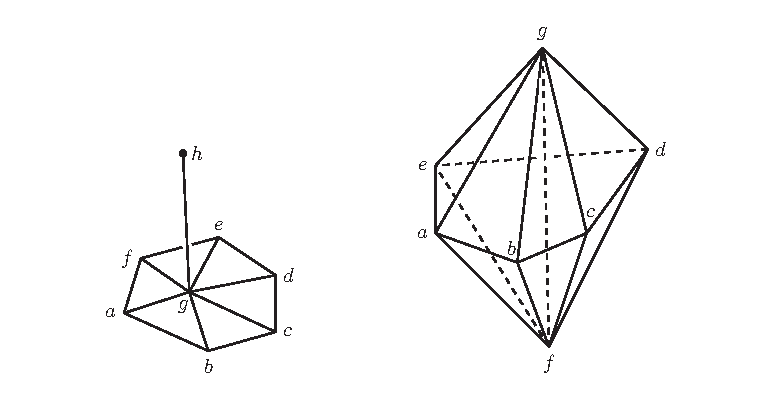
\includegraphics[width=.96\textwidth]{figures/8-2-1-2.pdf}
\caption*{图 8.2.1（左）与图 8.2.2（右）}
\end{figure}

\entry{引理}{8.2.10}设 $s$ 是复形 $K$ 的单形，则
\[
\overline{\operatorname{St}}s=s*\operatorname{Lk}s,\qquad
\overline{\operatorname{St}}s-\operatorname{St}s=\Bd s*\operatorname{Lk}s.
\]
这里把 $s,\Bd s,\operatorname{Lk}s$ 同时看作子空间和子复形。为使链环或边界为空时公式仍成立，约定 $K*\varnothing=\varnothing*K=K$。

\textbf{证明：}第一个等式直接来自定义：闭星形邻域由 $s*t$ 及其面组成，链环由相应的面 $t$ 组成。若一个单形位于闭星形邻域而不在开星形邻域中，它必为某个 $s*t$ 的面 $s'*t'$，其中 $s'$ 是 $s$ 的真面，$t'$ 是 $t$ 的面。因为 $t$ 在链环中，$t'$ 也在链环中，所以 $s'*t'$ 位于 $\Bd s*\operatorname{Lk}s$。反过来，每个这样的单形都在闭星形邻域中而不在开星形邻域中。\hfill$\square$

下面的定义推广定义 8.2.1，将在习题 2 中使用。

\entry{定义}{8.2.11}对拓扑空间 $X,Y$，定义 $X*Y$ 为 $X\times Y\times I$ 的商空间，其中把每个集合 $x\times Y\times0$ 压成一点，把每个 $X\times y\times1$ 压成一点。

\sourcepage{449--450}
\subsection*{习题}
\begin{enumerate}
\item 设 $s$ 是图 8.2.2 中的单形 $fg$。描述 $\widehat s*\operatorname{Lk}s$、$\widehat s*\Bd s$ 以及 $\Bd s*\operatorname{Lk}s$。
\item \begin{enumerate}[label=(\alph*)]
\item 证明 $i(x)=x\times Y\times0$ 和 $j(y)=X\times y\times1$ 分别定义 $X,Y$ 到 $X*Y$ 的嵌入。
\item 若 $X\approx X'$ 且 $Y\approx Y'$，证明 $X*Y\approx X'*Y'$。
\item 证明 $X*Y\approx Y*X$。
\end{enumerate}
\item 〔*〕证明存在分裂短正合列
\[0\to\widetilde H_{p+1}(X*Y)\to\widetilde H_p(X\times Y)
\to\widetilde H_p(X)\oplus\widetilde H_p(Y)\to0.\]
\item 〔*〕证明 $(X*Y)*Z\approx X*(Y*Z)$。〔提示：看似直接的证明并不奏效。下列两组商映射所实施的粘合不同：
\[
(X\times Y\times I_1)\times Z\times I_2\to(X*Y)\times Z\times I_2\to(X*Y)*Z,
\]
\[
X\times(Y\times Z\times I_2)\times I_1\to X\times(Y*Z)\times I_1\to X*(Y*Z).
\]
应在 $X\times Y\times Z\times\Delta_2$ 上引入以下等价关系：
\[
\begin{array}{ll}
(x,y,z,w)\sim(x',y,z,w),&w\in\epsilon_1\epsilon_2,\\
(x,y,z,w)\sim(x,y',z,w),&w\in\epsilon_0\epsilon_2,\\
(x,y,z,w)\sim(x,y,z',w),&w\in\epsilon_0\epsilon_1.
\end{array}
\]
记商空间为 $W$，商映射为 $\pi$。令 $f:I_1\times I_2\to\Delta_2$ 把 $t\times I_2$ 线性映到从 $t\in\epsilon_0\epsilon_1=[0,1]$ 到 $\epsilon_2$ 的线段。证明复合
\[
X\times Y\times Z\times I_1\times I_2
\xrightarrow{\mathrm{id}\times f}X\times Y\times Z\times\Delta_2\xrightarrow{\pi}W
\]
实施的粘合与前面第一组商映射相同，从而 $W\approx(X*Y)*Z$。再证明 $W\approx X*(Y*Z)$。〕
\item 设 $K,L$ 各为一个三角形。它们的联结是什么？
\item 把数字 $8$ 的形状写成两个单形的联结。
\end{enumerate}
